\documentclass[
10pt, % Main document font size
a4paper, % Paper type, use 'letterpaper' for US Letter paper
oneside, % One page layout (no page indentation)
%twoside, % Two page layout (page indentation for binding and different headers)
headinclude,footinclude, % Extra spacing for the header and footer
BCOR5mm, % Binding correction
]{scrartcl}

\usepackage{listings}
\usepackage{color}
%\usepackage{biblatex}

\definecolor{dkgreen}{rgb}{0,0.6,0}
\definecolor{gray}{rgb}{0.5,0.5,0.5}
\definecolor{mauve}{rgb}{0.58,0,0.82}

\lstset{frame=tb,
	language={},
	aboveskip=3mm,
	belowskip=3mm,
	showstringspaces=false,
	columns=flexible,
	basicstyle={\small\ttfamily},
	numbers=none,
	numberstyle=\tiny\color{gray},
	keywordstyle=\color{blue},
	commentstyle=\color{dkgreen},
	stringstyle=\color{mauve},
	breaklines=true,
	breakatwhitespace=true,
	tabsize=3
}

\usepackage{german}


%usepackage[utf8]{inputenc}
%\usepackage{geometry}
\usepackage[german,onelanguage,linesnumbered, ruled]{algorithm2e}
\SetAlFnt{\small}
\SetAlCapFnt{\large}
\SetAlCapNameFnt{\large}
%\usepackage{algpseudocode}


%%%%%%%%%%%%%%%%%%%%%%%%%%%%%%%%%%%%%%%%%
% Arsclassica Article
% Structure Specification File
%
% This file has been downloaded from:
% http://www.LaTeXTemplates.com
%
% Original author:
% Lorenzo Pantieri (http://www.lorenzopantieri.net) with extensive modifications by:
% Vel (vel@latextemplates.com)
%
% License:
% CC BY-NC-SA 3.0 (http://creativecommons.org/licenses/by-nc-sa/3.0/)
%
%%%%%%%%%%%%%%%%%%%%%%%%%%%%%%%%%%%%%%%%%

%----------------------------------------------------------------------------------------
%	REQUIRED PACKAGES
%----------------------------------------------------------------------------------------

\usepackage[
nochapters, % Turn off chapters since this is an article        
beramono, % Use the Bera Mono font for monospaced text (\texttt)
eulermath,% Use the Euler font for mathematics
pdfspacing, % Makes use of pdftex’ letter spacing capabilities via the microtype package
dottedtoc % Dotted lines leading to the page numbers in the table of contents
]{classicthesis} % The layout is based on the Classic Thesis style

\usepackage{arsclassica} % Modifies the Classic Thesis package

\usepackage[T1]{fontenc} % Use 8-bit encoding that has 256 glyphs

\usepackage[utf8]{inputenc} % Required for including letters with accents

\usepackage{graphicx} % Required for including images
\graphicspath{{Figures/}} % Set the default folder for images

\usepackage{enumitem} % Required for manipulating the whitespace between and within lists

\usepackage{lipsum} % Used for inserting dummy 'Lorem ipsum' text into the template

\usepackage{subfig} % Required for creating figures with multiple parts (subfigures)

\usepackage{amsmath,amssymb,amsthm} % For including math equations, theorems, symbols, etc

\usepackage{varioref} % More descriptive referencing

%----------------------------------------------------------------------------------------
%	THEOREM STYLES
%---------------------------------------------------------------------------------------

\theoremstyle{definition} % Define theorem styles here based on the definition style (used for definitions and examples)
\newtheorem{definition}{Definition}

\theoremstyle{plain} % Define theorem styles here based on the plain style (used for theorems, lemmas, propositions)
\newtheorem{theorem}{Theorem}

\theoremstyle{remark} % Define theorem styles here based on the remark style (used for remarks and notes)

%----------------------------------------------------------------------------------------
%	HYPERLINKS
%---------------------------------------------------------------------------------------

\hypersetup{
%draft, % Uncomment to remove all links (useful for printing in black and white)
colorlinks=true, breaklinks=true, bookmarks=true,bookmarksnumbered,
urlcolor=webbrown, linkcolor=RoyalBlue, citecolor=webgreen, % Link colors
pdftitle={}, % PDF title
pdfauthor={\textcopyright}, % PDF Author
pdfsubject={}, % PDF Subject
pdfkeywords={}, % PDF Keywords
pdfcreator={pdfLaTeX}, % PDF Creator
pdfproducer={LaTeX with hyperref and ClassicThesis} % PDF producer
} % Include the structure.tex file which specified the document structure and layout

\hyphenation{Fortran hy-phen-ation} % Specify custom hyphenation points in words with dashes where you would like hyphenation to occur, or alternatively, don't put any dashes in a word to stop hyphenation altogether

%----------------------------------------------------------------------------------------
%	TITLE AND AUTHOR(S)
%----------------------------------------------------------------------------------------

\title{\normalfont\spacedallcaps{Projektaufgabe AE}} % The article title

\subtitle{Remove Duplicates - Spotify playlist cleaner} % Uncomment to display a subtitle

\author{\spacedlowsmallcaps{Raphael Drechsler}} % The article author(s) - author affiliations need to be specified in the AUTHOR AFFILIATIONS block

\date{} % An optional date to appear under the author(s)

%----------------------------------------------------------------------------------------

\begin{document}

%----------------------------------------------------------------------------------------
%	HEADERS
%----------------------------------------------------------------------------------------

\renewcommand{\sectionmark}[1]{\markright{\spacedlowsmallcaps{#1}}} % The header for all pages (oneside) or for even pages (twoside)
%\renewcommand{\subsectionmark}[1]{\markright{\thesubsection~#1}} % Uncomment when using the twoside option - this modifies the header on odd pages
\lehead{\mbox{\llap{\small\thepage\kern1em\color{halfgray} \vline}\color{halfgray}\hspace{0.5em}\rightmark\hfil}} % The header style

\pagestyle{scrheadings} % Enable the headers specified in this block

%----------------------------------------------------------------------------------------
%	TABLE OF CONTENTS & LISTS OF FIGURES AND TABLES
%----------------------------------------------------------------------------------------

%\maketitle % Print the title/author/date block
{ \centering
{ \par}\
 \linebreak
\linebreak 
\linebreak
\linebreak
\linebreak
%\centering

\includegraphics[width=0.55\columnwidth]{htwLogo} 
\linebreak
\linebreak
\linebreak
\linebreak 
 % inline
{\fontsize{14}{16}\selectfont \center Fakultät Informatik, Mathematik und\\Naturwissenschaften\\Studiengang Informatik Master\par}\
 \linebreak
{\fontsize{18}{20}\selectfont \center \textbf{Projektarbeit zur Vorlesung Computermusik}\par}\
{\fontsize{20}{22}\selectfont \center \textbf{BrandtBrauerFrick.hs} \par}\
\linebreak
\linebreak
\linebreak
\linebreak 
\linebreak
\linebreak 
\linebreak 
{\fontsize{14}{16}\selectfont  \begin{tabular}{rl}
 	\textbf{Autoren:} & Nico Mehlhose, Raphael Drechsler\\ 
 	\textbf{Abgabedatum:} & 01.02.2019 \\ 
 \end{tabular}
\par}
\par}
\pagebreak
\setcounter{tocdepth}{2} % Set the depth of the table of contents to show sections and subsections only

%\tableofcontents % Print the table of contents
%\listoffigures % Print the list of figures
%\listoftables % Print the list of tables




%----------------------------------------------------------------------------------------

\newpage % Start the article content on the second page, remove this if you have a longer abstract that goes onto the second page

%----------------------------------------------------------------------------------------
%	INTRODUCTION
%----------------------------------------------------------------------------------------
\section{Abstract}\
Raph: \\
{\color{red}\textbf{TODO}} Wirkung? Klar machen!\\

\textbf{BrandtBrauerFrick.hs}

\noindent Brandt Brauer Frick ist ein Techno-Projekt aus Berlin.
Die Basis des Projekts bilden Klänge aus dem Instrumentarium der
klassischen Musik, welche anfangs gesampelt, später in einem zehnköpfigen
Ensemble auch live vorgeführt wurden.\cite{Wiki}\\ 

\noindent Ziel des Projektes:\\
Die Umsetzung des Songs ''Pretend'' von Brandt Brauer Frick entweder in
Tidal oder Euterpea. Dabei Orientierung an der Live-Aufführung
(https://www.youtube. com/watch?v=KCpLXpMB7F8).\\


\noindent Herausforderungen:
\begin{itemize}
	\item Evaluation ob Tidal oder Euterpea genutzt werden soll:
	\item Untersuchung der Frage ob klassische Klänge am ehesten in Euterpea oder
	Tidal nutzbar sind. (Durch repetitiven Charakter des Liedes würde sich Tidal zur
	Live-Vorführung eignen)
	\item Analyse der einzelnen musikalischen Bausteine und deren Implementierung.
\end{itemize}

\section{Tidal oder Euterpea}\
Nico\\
Dieses Thema soll sich um die Evaluation zwischen Tidal und Eutherpea handeln.\\
Unsere Entscheidung Tidal zu nehmen beruht gewiss nicht auf einer zufälligen Entscheidung. In diese Entscheidung ist der Programmieraufwand, vorhandenen Informationen
und die Möglichkeit den Synthesizer zu erweitern.\\
Bei dem Programmieraufwand wird sehr schnell klar, dass durch das Lied \textit{Pretent} von BrandBrauerFrick Tidal besser geeignet ist als Euterpea. Der erste Gesichtspunkt
der betrachtet wurde ist die Repetetivität des Songs, welcher in Euterpea zwar auch umsetzbar ist aber in Tidal von Anfang an gegeben ist, da Tidal die Sounds immer in einem
Loop abspielt. Bei den vorhandenen Informationen stellt sich heraus, dass es keine Offiziellen Notenblätter für das Lied Onlinegibt, wodurch Euterpea etwas an Bedeutung verliert, da Euterpea für genaue Notenbestimmungen perfekt geeignet wäre. Da dieser Fakt aber nicht vorliegt, kann das selbe Maß an Genauigkeit auch mit Tidal erreicht werden.\\
Der letzte und für uns wichtigste Punkt war die Erweiterbarkeit der Sounds. Die Wichtigkeit darin besteht in der entfremdeten Benutzung der Musikinstrumente in dem Lied.
In Eutherpea haben wir nach einiger Recherche keinen weg gefunden Sounds hinzuzufügen um diese später zu verwenden. In Tidal allerdings existiert diese Möglichkeit mittels
des Befehl \textit{}. Mit diesem Befehl lässt sich ein Verzeichnis in Tidal integrieren.
%~dirt.loadSoundFiles("full/path/to/directory/*") noch in textit einfügen
\section{Analyse des Stücks Pretend - Allgemein}\
\textit{Abschnitt bearbeitet von: Raphael Drechsler}\\

\noindent Tonart: Gm\\

\noindent Tempo: 130bpm.
\begin{lstlisting}
setcps (130/60/4)
\end{lstlisting}

\noindent Globale Struktur:
\begin{figure}[h]
	\centering 
	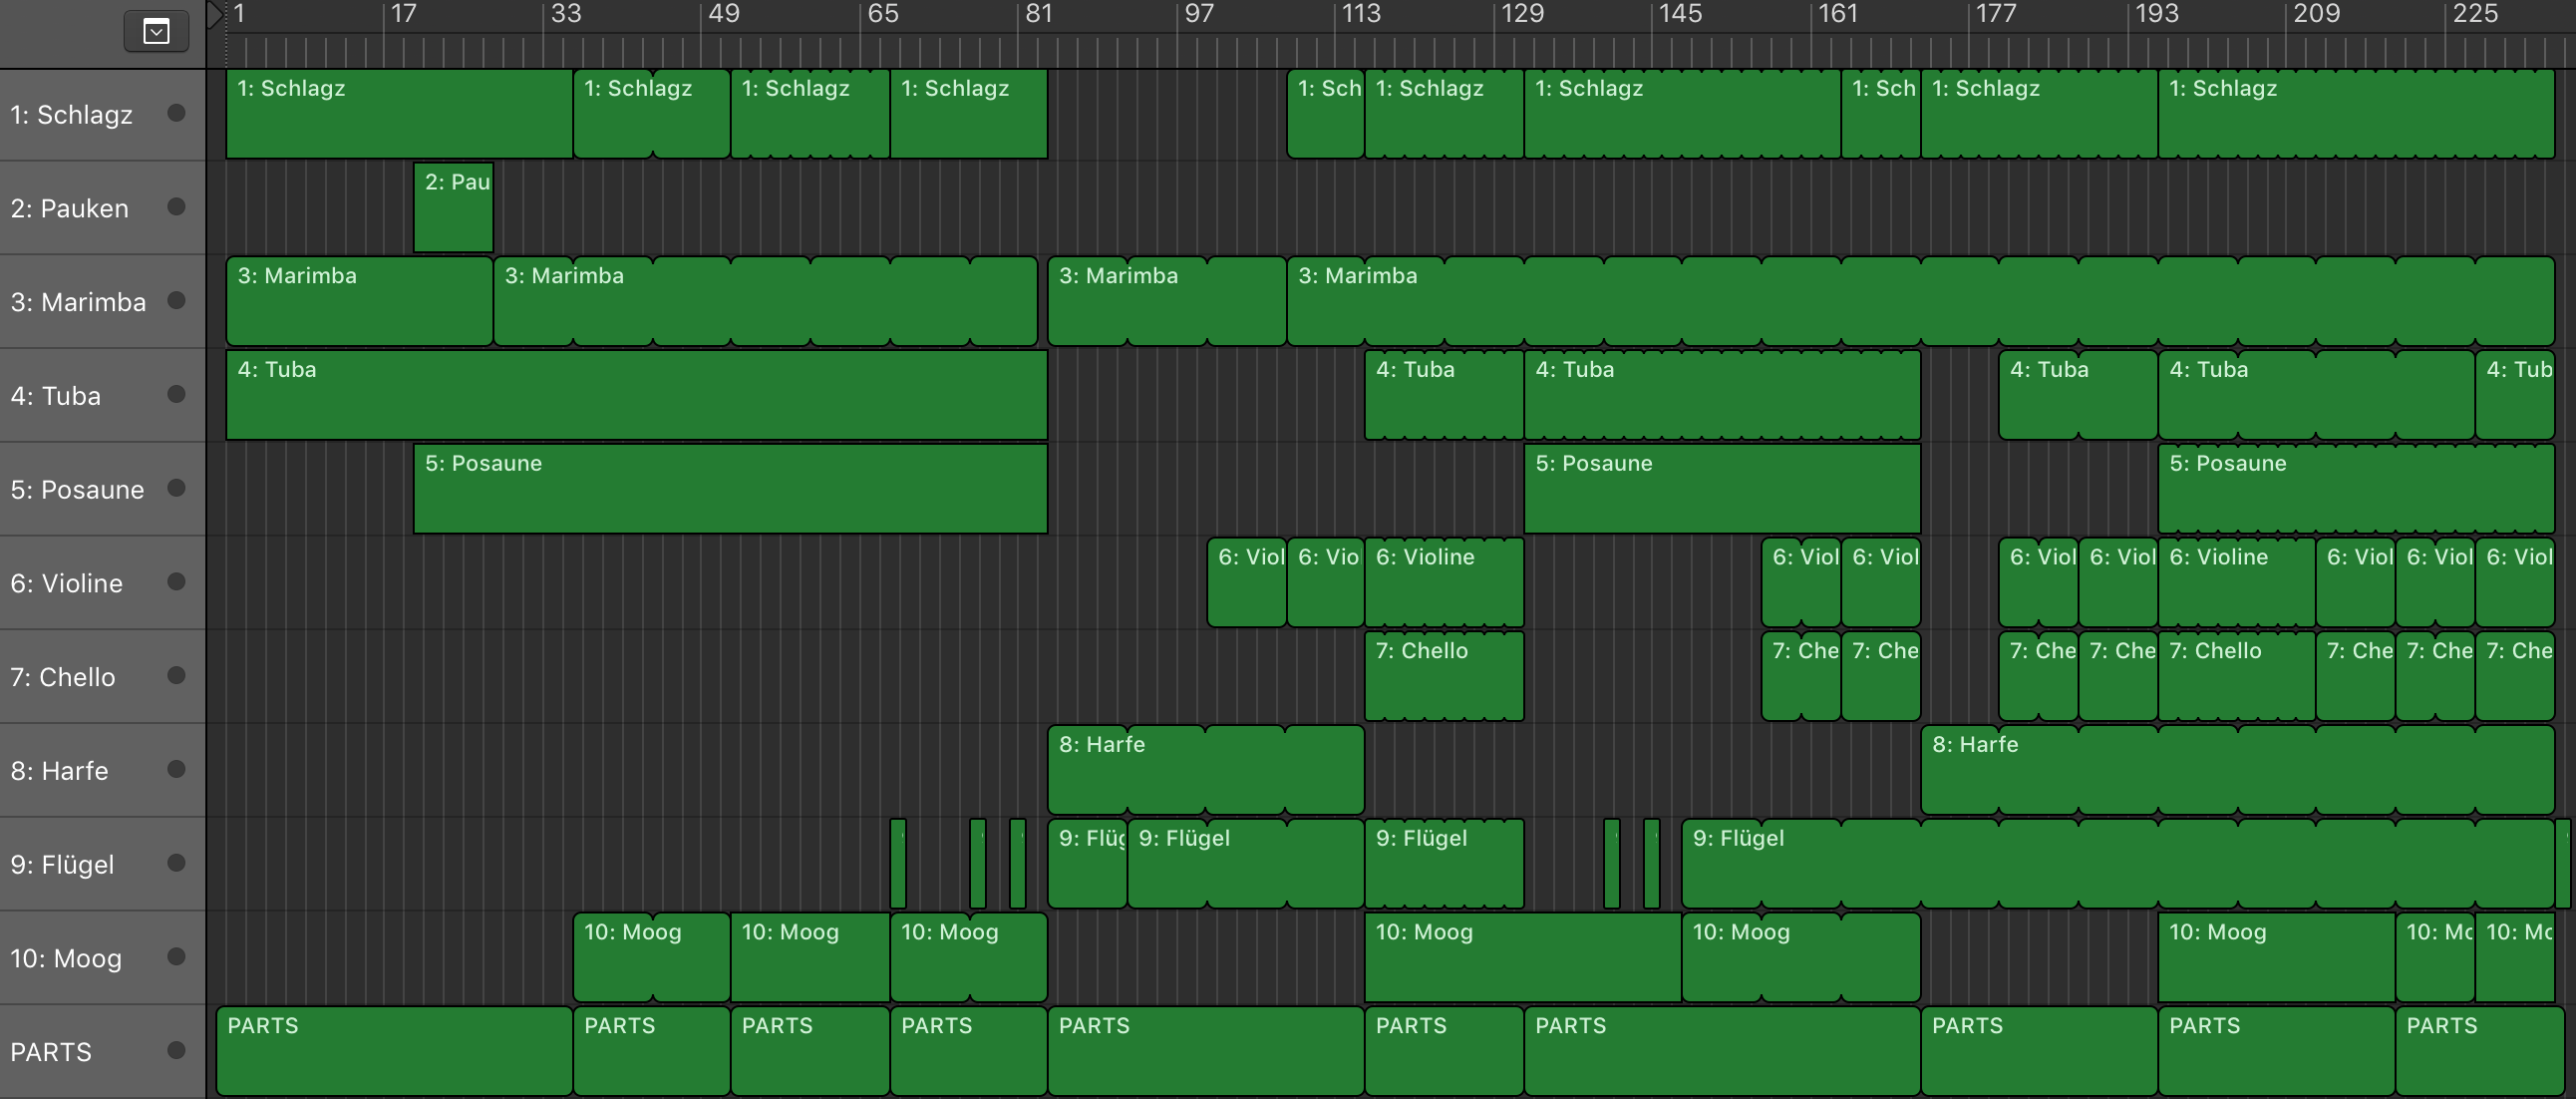
\includegraphics[width=0.99\columnwidth]{GlobaleStruktur} 
	\caption{Globale Struktur dargestellt als leere MIDI-Regionen in DAW}
\end{figure}

{\color{red}\textbf{TODO}}: Score?

\section{Analyse des Stücks Pretend}\
Im folgenden Abschnitt sollen die zehn Instrumentalisten untersucht werden.

\subsection{Instrument 0: Was ist pro Instrument TODO?}
{\color{red}\textbf{TODO}}: Nach Bearbeitung Hilfskapitel entfernen.\\

Raph.\\
Welche Figuren?
- Welche Wirkung?
- Welche Noten?\\

Nico\\
Wie klingt das Instrument?\\
- Wie klingt das live? Einzelne Bestandteile? (Marimba gespielt mit Holzsticks und verschiedene Kuhglocken)
- Wie klingt das in welcher Figur? (zB. BD laut, leise)
- Welchen Klang wählen (evaluation - SD-Instrument nutzbar?, WAV suchen/selber aufnehmen, Instrument coden)\\

\subsection{Instrument 1: Schlagzeug}
\subsubsection{Figuren}
{\color{orange}\textbf{WIP}} \\

\textbf{Figur 1}\\
treibender Grundrhytmus, steigende Lautstärke BD
\begin{figure}[h]
	\centering 
	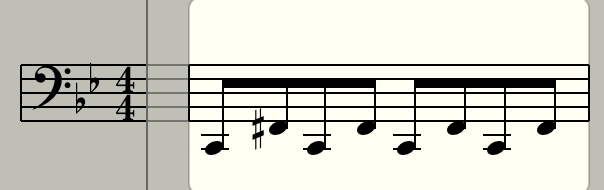
\includegraphics[width=0.35\columnwidth]{Drum_Fig1} 
	\caption{Schlagzeug Figur 1}
\end{figure}

\begin{lstlisting}
d1 $ sound "[bd hh]*4"
\end{lstlisting}

\noindent \textbf{Figur 2}\\
Wie 1 mit Fills\\
{\color{red}\textbf{TODO}} Logic, Noten, Code oder Absicht und Programmlogik\\

\noindent \textbf{Figur 3}\\
Wie 1 und 2, noch mehr Fills\\
{\color{red}\textbf{TODO}} Logic, Noten, Code oder Absicht und Programmlogik\\

\noindent \textbf{Figur 4}\\
Wie 1, keine Fills auf hh,
zyklische Bewegung auf rim: Angenommen 5Schläge Pro Takt.

\begin{lstlisting}
d1 $ sound "[[bd hh]*4, rm*5]"
d1 $ sound "[[bd hh]*4, rm rm rm rm ~]"
\end{lstlisting}

um einen Cycle draus zu machen rand nutzen:

\begin{lstlisting}
d1 $ sound "[[bd hh]*4, rm rm rm rm rm?]"
\end{lstlisting}

oder

\begin{lstlisting}
d1 $ slow 2 $ stack [
sound "[bd hh]*8",
fastcat[sound "[rm rm rm rm rm]", sound "[rm rm rm rm ~]"]
]
\end{lstlisting}



\noindent \textbf{Figur 5}\\
Nur Triolen auf Rim.
\begin{lstlisting}
d1 $ slow 2 $ fastcat[sound "[rm rm rm rm rm]", sound "[rm rm rm rm ~]"]
\end{lstlisting}


\noindent \textbf{Figur 6}\\
Wie Figur 4 aber kräftig gespielt.\\

\noindent \textbf{Figur 7}\\
Treibentder Rhytmus, viele Fills -> Was analoges zu Figur 3\\
{\color{red}\textbf{TODO}} Logic, Noten, Code oder Absicht und Programmlogik\\

\noindent Im Ablauf: \textbf{Block mit Figur 6}\\

\noindent \textbf{Figur 8}\\
Wie 4 aber ohne BD.
\begin{lstlisting}
d1 $ slow 2 $ stack [
sound "[~ hh]*8",
fastcat[sound "[rm rm rm rm rm]", sound "[rm rm rm rm ~]"]
]
\end{lstlisting}

\noindent Im Ablauf: \textbf{Block mit Figur 6}

\subsubsection{Klangbild}
Sound BD:\\
Sound HH:\\

Fig1: Problem: bd wird lauter, Lösung:\\
\begin{lstlisting}
Nicos Code: d1 $ whenmod 200 100 (|*|gain "0.8 0.7 0.8 0.7 0.8 0.7 0.8 0.7" ) $ sound "[bd hh]*4" # gain "0.5 0.7 0.5 0.7 0.5 0.7 0.5 0.7" # midinote 58
--Idee: d1 $ slow 2 $ sound "[bd hh]*8" #gain "<0.7 0.9 1.1 1.3>"
\end{lstlisting}

Fig4:\\
Sound Rim:\\
Nico: selber bauen da keine hölzernen klänge vorhanden sind

Fig6:\\
irgendwas mit gain?\\



Töne: hh, bd (dumpf, wenig knackig)\\
rim

\subsection{Instrument 2: Pauken}
\subsubsection{Figuren}
{\color{red}\textbf{OFFEN}} \\
{\color{red}\textbf{TODO}}
(Hierzu Studio-Version hören)\\

\subsubsection{Klangbild}
3 Kesselpauken

\subsection{Instrument 3: Marimba}
\subsubsection{Figuren}
{\color{red}\textbf{OFFEN}} \\
{\color{red}\textbf{TODO}}\\
Aufbau beschreiben mit Glocken.\\
Random-Funktion benötigt

\subsubsection{Klangbild}
Holzsticks auf Marimba in verschiednenen Tonhöhen wobei eher rhythmisch als melodisch eingesetzt, dazu Kuh-Glocken bereitstellen für Random-Funktion

\subsection{Instrument 4: Tuba}
\subsubsection{Figuren}
{\color{orange}\textbf{WIP}} \\

\noindent\textbf{Figur 1}\\
Figur über einen Takt. Schlag auf Tuba-Mundstück als rhythmisches Element auf zweite Zählzeit im Takt.\\
\begin{figure}[h]
	\centering 
	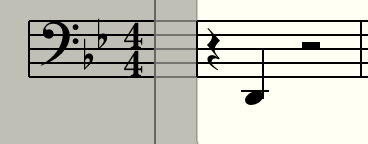
\includegraphics[width=0.25\columnwidth]{Tuba_Fig1} 
	\caption{Tuba Figur 1}
\end{figure}

\begin{lstlisting}
d1 $ sound "[~ sn ~ ~]"
\end{lstlisting}

\subsubsection{Figuren}
\textbf{Figur 2}\\
Figur über 2 Takte. Instrumentalist bläst in die Tuba ohne dass die Lippen vibrieren, um ein Rauschen zu erzeugen. Pause am Ende der Figur als Atempause angenommen. 

\begin{figure}[h]
	\centering 
	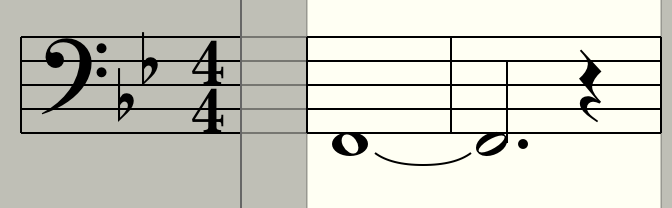
\includegraphics[width=0.25\columnwidth]{Tuba_Fig2} 
	\caption{Tuba Figur 2}
\end{figure}

\begin{lstlisting}
--Idee: sound, der 2 Takte dauert alle 2 Takte 1x anpsielen
d1 $ sound "blasesoundTuba"
\end{lstlisting}

\noindent\textbf{Figur 3}\\
Wie Figur 1, hier allerdings kurzes tonloses Pusten stoßweise gespielt anstelle von Schlag auf Mundstück.\\

\noindent\textbf{Figur 4}\\
Tiefe Töne durch Tuba, Tonhöhe nicht entscheidend und fast nicht mehr wahrnehmbar. Gefühl von Bedrohung. Rollt langsam an\\
{\color{red}\textbf{TODO}} Logic, Noten, Code\\

\noindent\textbf{Figur 5}\\
Wie Figur 4, kräftig ausgespielt.\\

\noindent\textbf{Figur 6}\\
Wie Figur 5, maximal kraftvoll ausgespielt. Eine Oktave höher gespielt daher Tonhöhe der einzelnen Töne gut erkennbar.\\
{\color{red}\textbf{TODO}} Code

\subsubsection{Klangbild}

Figur 1 Sound:
\begin{lstlisting}
Code Nico: d1 $ sound "~ bd ~ ~" # midinote 15
\end{lstlisting}

Fig2:
Nico: geht nicht da kein sound mit gleichbleibender schwingung (scheibenwischer)

schlagen, blasen(impulsartig,durchgehend), spielen(tief, hoch)\\
\begin{lstlisting}
Nico: d1 $ sound "[sax ~ ~ hh]" # speed 0.35 # midinote 55 # gain "[1 0]" # cut 1 \\
d1 $ sound "[trump ~ ~ hh]" # speed 0.05 # midinote 55 # gain "[0.7 0]" # cut 1\\\\

das ist das naechste was ich an den sound rankomme
da wir aber noch 3 weitere gute tubasounds brauchen wuerde ich die mir denke auch lieber ziehen wollen
\end{lstlisting}



\subsection{Instrument 5: Posaune}
\subsubsection{Figuren}
{\color{green}\textbf{FERTIG}} \\

\noindent\textbf{Figur 1}\\
Figur über einen Takt. Kurzes, tonloses Pusten in die Posaune. Stoßweise gespielt als rhythmisches Element auf letzte Achtelnote im Takt.\\
\begin{figure}[h]
	\centering 
	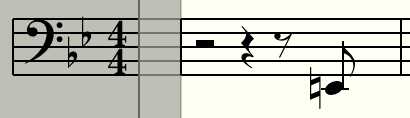
\includegraphics[width=0.25\columnwidth]{Posaune_Fig1} 
	\caption{Posaune Figur 1}
\end{figure}

\begin{lstlisting}
d1 $ sound "[][[][~ sn]]"
\end{lstlisting}


\noindent\textbf{Figur 2}\\
Erzeugen von Rauschen analog zu Figur 2 - Tuba. Dabei Lautstärke zum Ende des Stückes hin zunehmend.
\begin{lstlisting}
--Idee: sound, der 2 Takte dauert alle 2 Takte 1x anpsielen
--Frage: Lautstaerke?
d1 $ sound "blasesoundPosaune"
\end{lstlisting}

\subsubsection{Klangbild}
blasen(impulsartig,durchgehend)

\subsection{Instrument 6: Violine}
\subsubsection{Figuren}
{\color{orange}\textbf{WIP}} \\
\noindent\textbf{Figur 1}\\
\begin{figure}[h]
	\centering 
	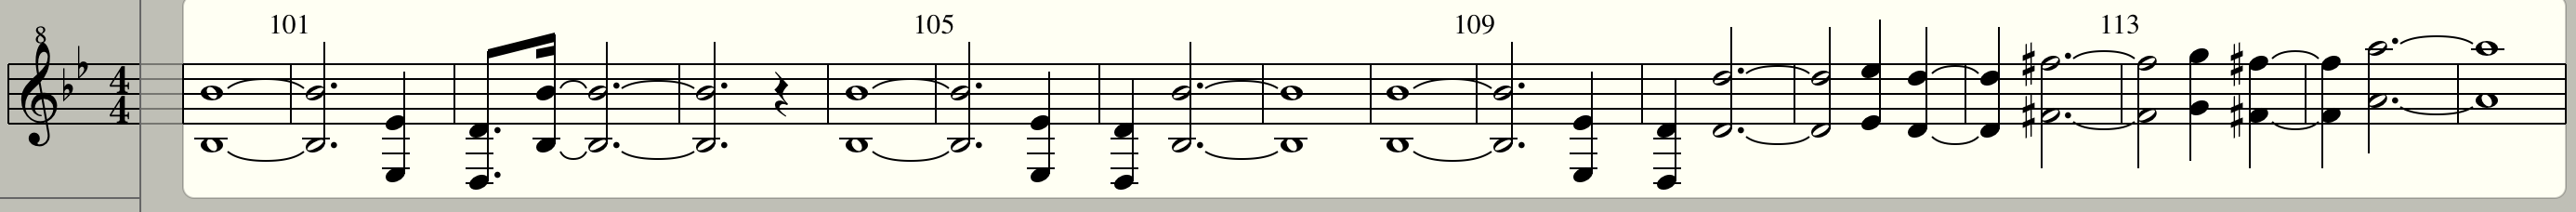
\includegraphics[width=0.99\columnwidth]{Violin_Fig1} 
	\caption{Violine Figur 1}
\end{figure}

\begin{lstlisting}
p "i6" $ slow 16 $ fastcat [
midinote "[82][][][][][][][75][74][82][][][][][][]" # s "gtr",
midinote "[82][][][][][][][75][74][82][][][][][][]" # s "gtr",
midinote "[82][][][][][][][75][74][86][][][][][87][86]" # s "gtr",
midinote "[][90][][][][][91][90][][93][][][][][][]" # s "gtr"
] # room 0.85 # sz 0.8 # orbit 1 #gain 0.9
\end{lstlisting}

\noindent\textbf{Figur 2}\\
\begin{figure}[h]
	\centering 
	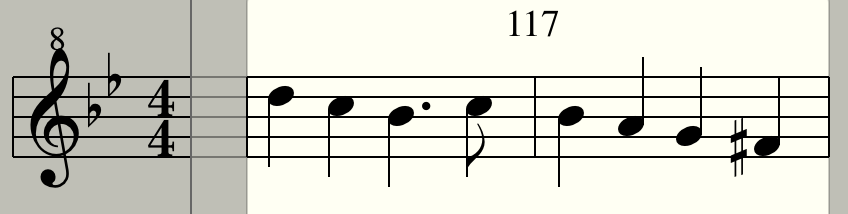
\includegraphics[width=0.3\columnwidth]{Violin_Fig2} 
	\caption{Violine Figur 2}
\end{figure}

\begin{lstlisting}
p "i6" $ slow 2 $ midinote "[[86][84][82][[][84]]][82 81 79 78]" # s "gtr"
\end{lstlisting}

{\color{red}\textbf{TODO}} weitere Figuren im hinteren Teil des Stückes

\subsubsection{Klangbild}
Ruhige Parts, Hektik (schnell gespielte Töne)


\subsection{Instrument 7: Chello}
\subsubsection{Figuren}
{\color{orange}\textbf{WIP}} \\
\noindent\textbf{Figur 1}\\
\begin{figure}[h]
	\centering 
	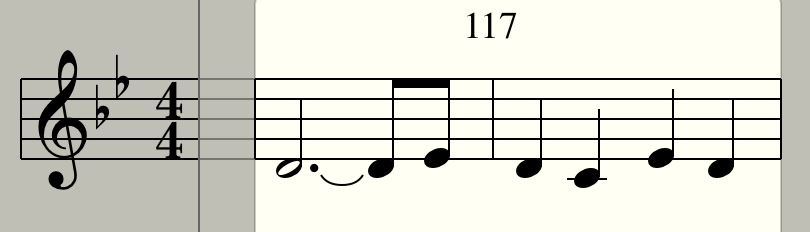
\includegraphics[width=0.3\columnwidth]{Chello_Fig1} 
	\caption{Chello Figur 1}
\end{figure}

\begin{lstlisting}
p "i7" $ slow 2 $ midinote "[[74][][][[][75]]][74 72 75 74]" # s "gtr"
\end{lstlisting}

\noindent\textbf{Figur 2}\\
{\color{red}\textbf{TODO}} 


{\color{red}\textbf{TODO}} weitere Figuren im hinteren Teil des Stückes

\subsubsection{Klangbild}
Ruhige Parts, Hektik (schnell gespielte Töne)


\subsection{Instrument 8: Harfe}
\subsubsection{Figuren}
{\color{green}\textbf{vorerst FERTIG}} \\
\noindent\textbf{Figur 1}\\
{\color{red}\textbf{TODO}} Starke Annahme - hier vllt was mit Random aus Skala nehmen machen.
\begin{figure}[h]
	\centering 
	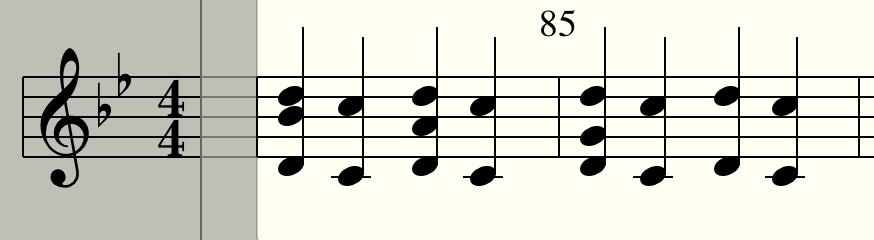
\includegraphics[width=0.3\columnwidth]{Harp_Fig1} 
	\caption{Harfe Figur 1}
\end{figure}

\begin{lstlisting}
d1 $ slow 2 $ stack [
	midinote "[74 72]*4" # s "gtr", 
	midinote "[62 60]*4" # s "gtr", 
	slow 2 $ fastcat [
		midinote "70 69" # s "gtr", 
		midinote "67" # s "gtr",
		midinote "70 69" # s "gtr", 
		midinote "66" # s "gtr"    
	]
]
\end{lstlisting}



\subsubsection{Klangbild}
...

\subsection{Instrument 9: Flügel}
\subsubsection{Figuren}
{\color{orange}\textbf{WIP}} \\
\noindent\textbf{Figur 1}\\
Nur ein Tiefer Ton.
\begin{figure}[h]
	\centering 
	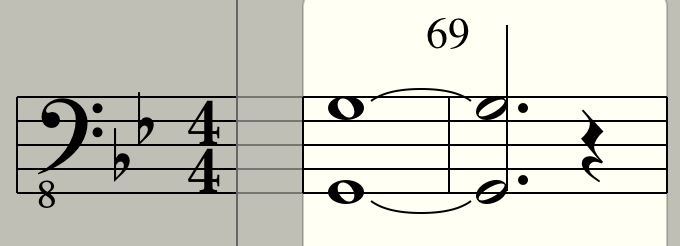
\includegraphics[width=0.3\columnwidth]{Flug_Fig1} 
	\caption{Flügel Figur 1}
\end{figure}

\begin{lstlisting}
p "i9" $ slow 2 $ stack[midinote "43 " #s "superpiano", midinote "55 " #s "superpiano"]
-- wie verknuepfen bzw. nur 1x spielen lassen?
\end{lstlisting}

\noindent \textbf{Figur 2}\\
\begin{figure}[h]
	\centering 
	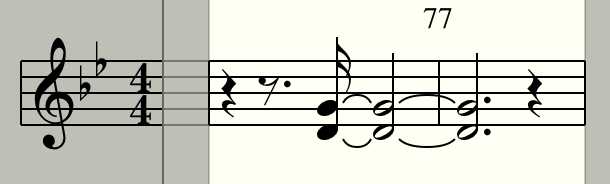
\includegraphics[width=0.3\columnwidth]{Flug_Fig2} 
	\caption{Flügel Figur 2}
\end{figure}\\
{\color{red}\textbf{TODO}} Code\\


\noindent \textbf{Figur 3}\\
{\color{red}\textbf{TODO}}Beschreibung\\
\begin{figure}[h]
	\centering 
	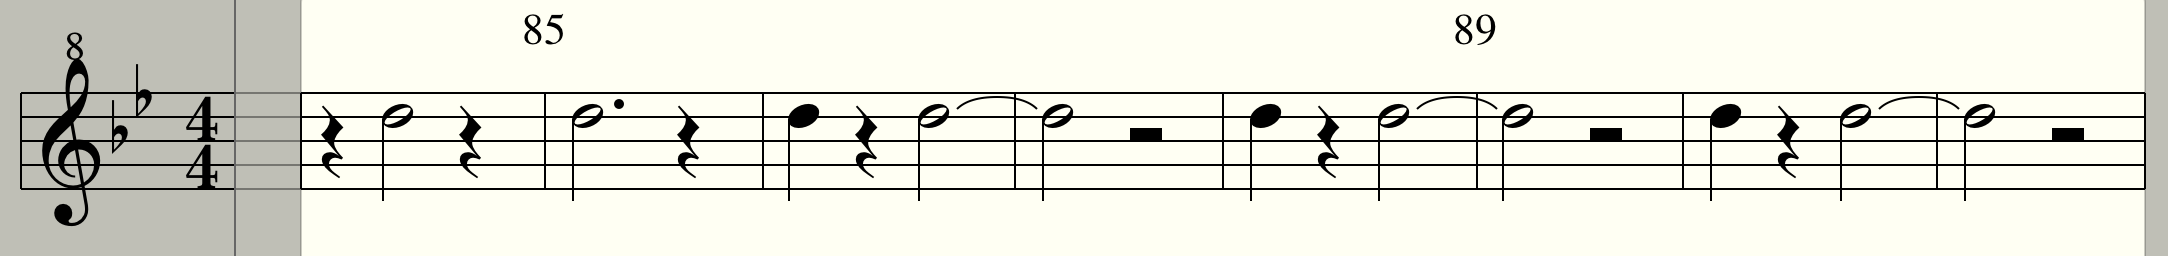
\includegraphics[width=0.9\columnwidth]{Flug_Fig3} 
	\caption{Flügel Figur 3}
\end{figure}
\begin{lstlisting}
p "i9" $ slow 2 $ midinote "[86 ~][86][~] [~] " # s "superpiano"  # room 0.5 # sz 0.83 # orbit 1 #gain "<0.65 0.7 0.75 0.8>"
\end{lstlisting}


\noindent \textbf{Figur 4}\\
{\color{red}\textbf{TODO}}Beschreibung\\
\begin{figure}[h]
	\centering 
	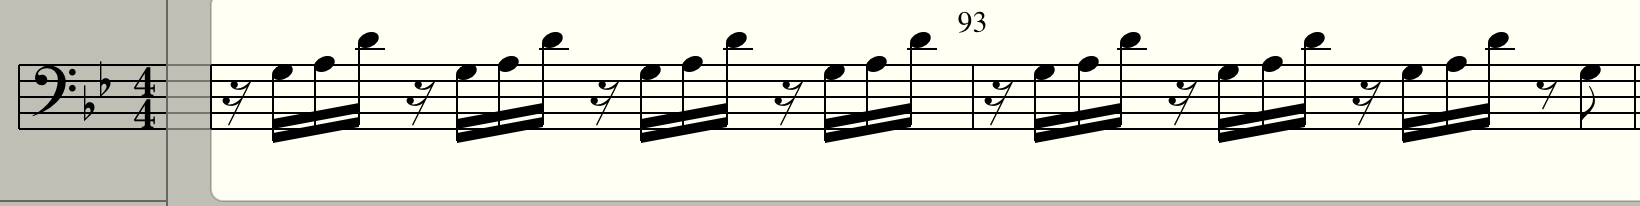
\includegraphics[width=0.9\columnwidth]{Flug_Fig4a} 
	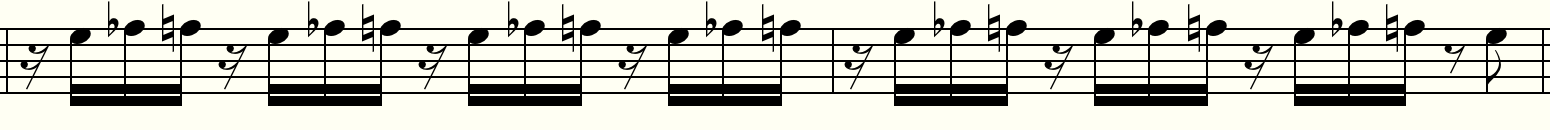
\includegraphics[width=0.9\columnwidth]{Flug_Fig4b} 
	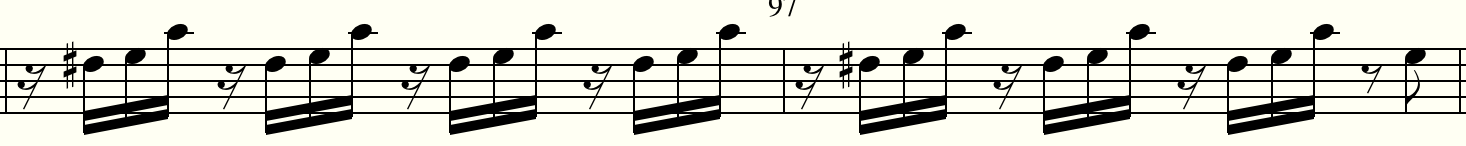
\includegraphics[width=0.9\columnwidth]{Flug_Fig4c} 
	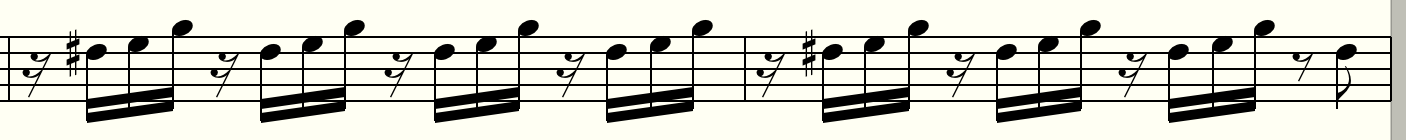
\includegraphics[width=0.9\columnwidth]{Flug_Fig4d} 
	\caption{Flügel Figur 4}
\end{figure}
\begin{lstlisting}
d1 $ slow 8 $ fastcat [
midinote "~ 67 69 74 ~ 67 69 74 ~ 67 69 74 ~ 67 69 74 ~ 67 69 74 ~ 67 69 74 ~ 67 69 74  ~ ~ 67 ~ " # s "superpiano",
midinote "~ 67 68 69 ~ 67 68 69 ~ 67 68 69 ~ 67 68 69 ~ 67 68 69 ~ 67 68 69 ~ 67 68 69  ~ ~ 67 ~ " # s "superpiano",
midinote "~ 66 67 72 ~ 66 67 72 ~ 66 67 72 ~ 66 67 72 ~ 66 67 72 ~ 66 67 72 ~ 66 67 72  ~ ~ 67 ~ " # s "superpiano",
midinote "~ 66 67 70 ~ 66 67 70 ~ 66 67 70 ~ 66 67 70 ~ 66 67 70 ~ 66 67 70 ~ 66 67 70  ~ ~ 66 ~ " # s "superpiano"
]
\end{lstlisting}
{\color{green}\textbf{OK}} \\


\noindent \textbf{Figur 5}\\
\begin{figure}[h]
	\centering 
	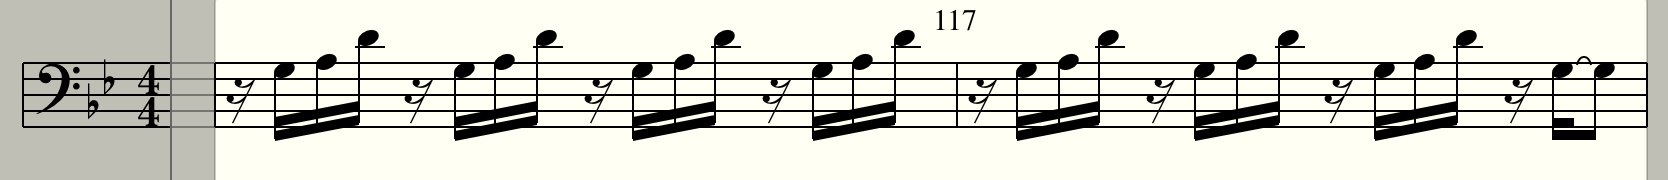
\includegraphics[width=0.9\columnwidth]{Flug_Fig5} 
	\caption{Flügel Figur 5}
\end{figure}
\begin{lstlisting}
d1 $ slow 2 $ midinote "~ 67 69 74 ~ 67 69 74 ~ 67 69 74 ~ 67 69 74 ~ 67 69 74 ~ 67 69 74 ~ 67 69 74  ~ ~ 67 ~ " # s "superpiano"
\end{lstlisting}
{\color{green}\textbf{OK}} \\

\subsubsection{Klangbild}
...


\subsection{Instrument 10: Moog Syntheziser}
\subsubsection{Figuren}
{\color{green}\textbf{vorerst FERTIG}} \\

\noindent\textbf{Figur 1}\\
Basslauf über 8 Takte.\\
\begin{figure}[h]
	\centering 
	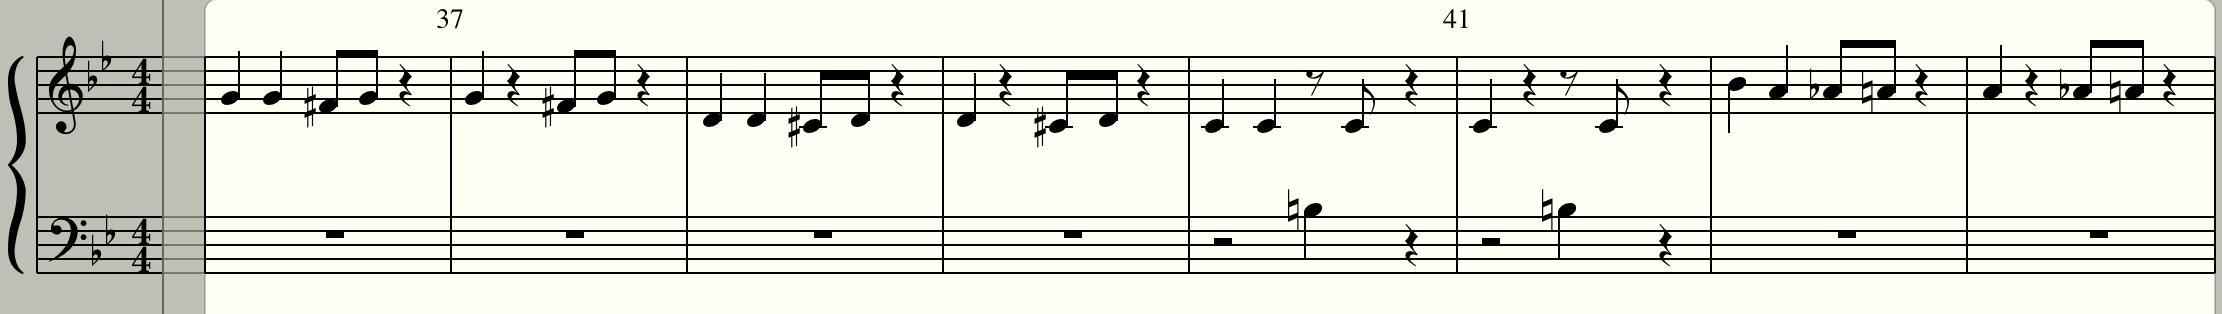
\includegraphics[width=1\columnwidth]{Bass_Fig1} 
	\caption{Moog Figur 1}
\end{figure}

\begin{lstlisting}
---Arbeitsstand
--2Takte
d1 $ midinote "[[55 55][54 55 ~ ~]]" # s "moog" # cut 1
--2Takte
d1 $ midinote "[[50 50][49 50 ~ ~]]" # s "moog" # cut 1
--2Takte
d1 $ midinote "[[48 48][47 48 ~ ~]]" # s "moog" # cut 1
--1 Takte
d1 $ midinote "[[58 57][56 57 ~ ~]]" # s "moog" # cut 1
--1 Takte
d1 $ midinote "[[57 ~][56 57 ~ ~]]" # s "moog" # cut 1

---Verbunden:
d1 $ slow 8 $ fastcat [midinote "[[55 55][54 55 ~ ~]]*2" # s "moog" # cut 1,
midinote "[[50 50][49 50 ~ ~]]*2" # s "moog" # cut 1,
midinote "[[48 48][47 48 ~ ~]]*2" # s "moog" # cut 1,
midinote "[[58 57][56 57 ~ ~]]  [[57 ~][56 57 ~ ~]]" # s "moog" # cut 1
]
\end{lstlisting}

\noindent\textbf{Figur 2}\\
Basslauf über einen Takt.
\begin{figure}[h]
	\centering 
	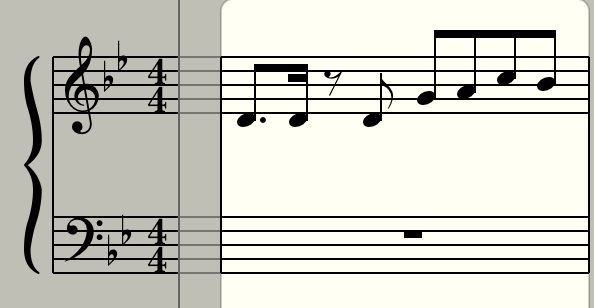
\includegraphics[width=0.3\columnwidth]{Bass_Fig2} 
	\caption{Moog Figur 2}
\end{figure}

\begin{lstlisting}
---Arbeitsstand
d1 $ midinote "[[[[50 ~ ~ 50]][~ 50]][55 57 60 58]]" # s "moog" # cut 1
\end{lstlisting}



\subsubsection{Klangbild}
...

\section{Performance}
TODO:\\
Spuren per Stack verbinden?\\

\begin{lstlisting}
--10 Instruments:
p "i1" $ sound "bd sd:1"
p "i2" $ sound "hh hh hh hh"
p "i3" $ sound "hh hh hh hh"
p "i4" $ sound "hh hh hh hh"
p "i5" $ sound "hh hh hh hh"
p "i6" $ sound "hh hh hh hh"
p "i7" $ sound "hh hh hh hh"
p "i8" $ sound "hh hh hh hh"
p "i9" $ sound "hh hh hh hh"
p "i10" $ sound "hh hh hh hh"
\end{lstlisting}
Konzept für Ablauf Performance?\\
Wie mehrtaktige Figuren mit every zusammenfassen?

Link zu den Soundfiles: http://virtualplaying.com/virtual-playing-orchestra/ \\
https://rhythm-lab.com/moog-rogue-bass/

\pagebreak

%----------------------------------------------------------------------------------------
%	BIBLIOGRAPHY
%----------------------------------------------------------------------------------------

\renewcommand{\refname}{\spacedlowsmallcaps{Literatur/Quellen}} % For modifying the bibliography heading

\bibliographystyle{unsrt}

\bibliography{biblo.bib} % The file containing the bibliography

%----------------------------------------------------------------------------------------

\end{document}